\section{Phân tích yêu cầu}

\subsection{Yêu cầu chức năng}

Các yêu cầu chức năng chính của hệ thống gồm: triển khai workload tại Sydney; sao lưu RDS và copy recovery point sang Singapore; replicate image và secret; phát hiện trạng thái không sẵn sàng của ba target group; khởi tạo workflow DR; dựng hạ tầng runtime; restore RDS; cập nhật cấu hình kết nối; scale ba ECS service; kiểm tra target health; tùy chọn tạo record Route~53 SECONDARY; gửi thông báo và hỗ trợ cleanup có kiểm soát.

Ứng dụng demo cung cấp các endpoint \texttt{/health}, \texttt{/products}, \texttt{/products/\{id\}}, \texttt{/auth} và \texttt{/order}. Endpoint health mở kết nối PostgreSQL, khởi tạo bảng \texttt{products} nếu cần và chạy \texttt{SELECT 1}. Endpoint product cho phép tạo, liệt kê và đọc bản ghi. Chức năng này đủ để kiểm chứng một recovery point có chứa dữ liệu được ghi trước backup.

\subsection{Yêu cầu phi chức năng}

\begin{itemize}
  \item \textbf{Khả năng phục hồi:} recovery point phải tồn tại ở Region độc lập; workflow phải kiểm tra hạ tầng, database và application health trước khi đánh dấu thành công.
  \item \textbf{Bảo mật:} database không public; credentials không hard-code; tài nguyên mã hóa; Security Group giới hạn luồng; IAM tách vai trò theo chức năng.
  \item \textbf{Tối ưu chi phí:} DR runtime không tồn tại thường trực; ECS khởi tạo desired count bằng 0; RDS chỉ xuất hiện sau restore.
  \item \textbf{Khả năng quan sát:} log ứng dụng dạng JSON, CloudWatch dashboard, Step Functions execution history, SNS notification và dead-letter queue.
  \item \textbf{Khả năng lặp lại:} hạ tầng khai báo bằng CloudFormation; package và deploy qua script PowerShell.
  \item \textbf{An toàn vận hành:} confirmation window, singleton lock, kiểm tra lại Primary trước cutover, safe test mặc định bỏ qua DNS và cleanup yêu cầu cờ xác nhận.
\end{itemize}

\section{Kiến trúc tổng thể}

Hình~\ref{fig:architecture-overall} trình bày kiến trúc tổng thể gồm Sydney Primary, Singapore DR, các luồng sao chép backup/image/secret và control plane tại Singapore. Record DNS SECONDARY chỉ được tạo khi workflow nhận đầu vào cho phép; cấu hình EventBridge và kịch bản kiểm thử hiện mặc định bỏ qua cutover để bảo vệ traffic đang phục vụ.

\begin{figure}[H]
  \centering
  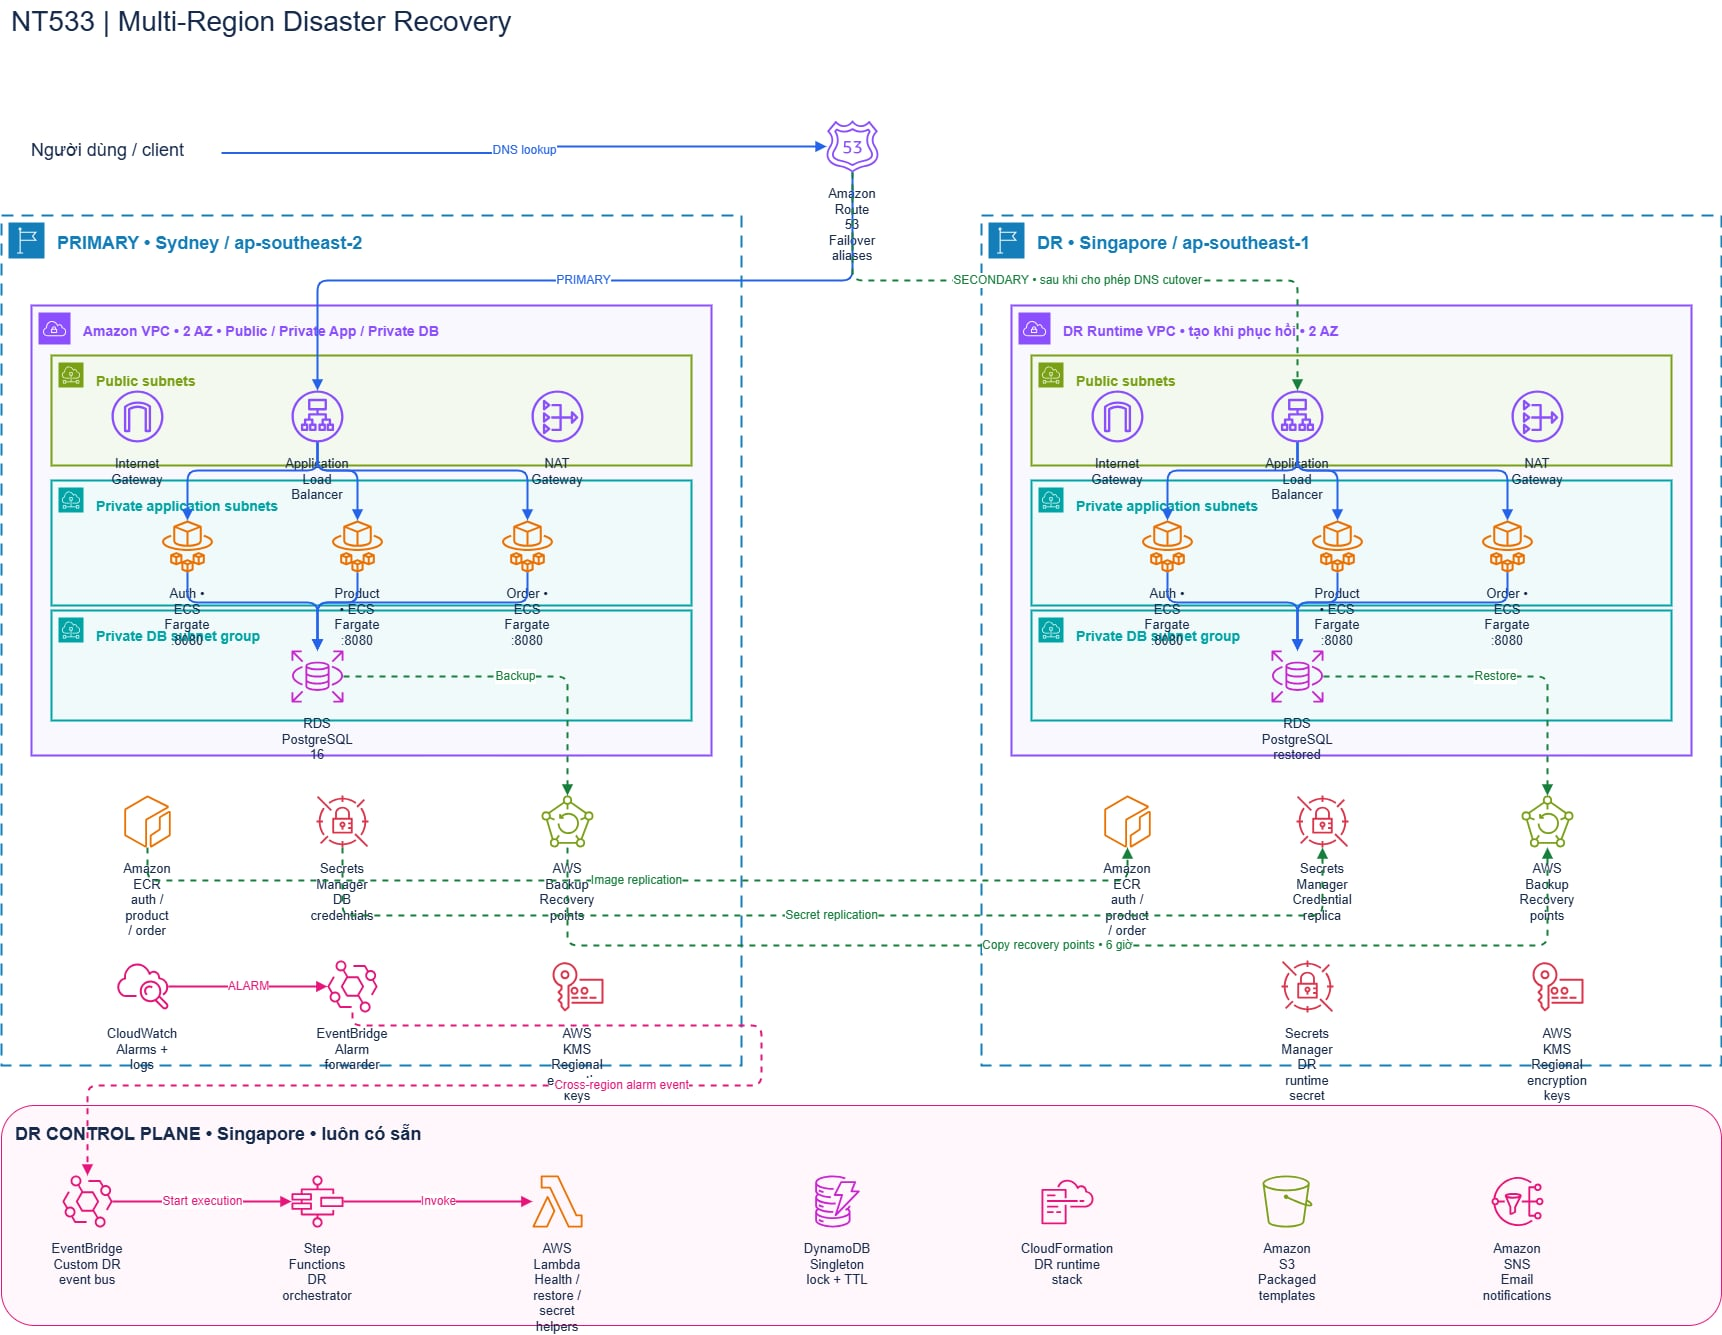
\includegraphics[width=\textwidth]{img/chapter3/nt533-architecture.jpg}
  \caption{Kiến trúc Multi-Region Disaster Recovery của NT533}
  \label{fig:architecture-overall}
\end{figure}

Luồng bình thường có thể tóm tắt như sau:

\begin{center}
\begin{tikzpicture}[node distance=9mm and 8mm, every node/.style={font=\small}, box/.style={draw, rounded corners, align=center, minimum height=9mm, fill=blue!5}, data/.style={draw, cylinder, shape border rotate=90, aspect=0.25, align=center, fill=green!8}, >=Latex]
\node[box] (client) {Client};
\node[box, right=of client] (dns) {Route 53\\PRIMARY};
\node[box, right=of dns] (alb) {ALB\\Sydney};
\node[box, right=of alb] (ecs) {ECS Fargate\\3 services};
\node[data, right=of ecs] (rds) {RDS\\PostgreSQL};
\draw[->] (client)--(dns);
\draw[->] (dns)--(alb);
\draw[->] (alb)--(ecs);
\draw[->] (ecs)--(rds);
\end{tikzpicture}
\end{center}

Song song với request path, AWS Backup tạo recovery point và copy sang Singapore; ECR replicate image theo prefix; Secrets Manager replicate credentials. Control plane DR tồn tại độc lập với runtime VPC, cho phép Region Singapore bắt đầu phục hồi ngay cả khi workload Sydney không truy cập được.

\section{Kiến trúc Primary Region}

\subsection{Mạng}

Template \path{cloudformation/primary/network.yaml} tạo VPC \texttt{10.10.0.0/16} trên hai AZ. Mỗi AZ có public, private application và private database subnet. Hai public subnet dùng chung route table có default route đến Internet Gateway. Hai application subnet dùng chung route table đi qua một NAT Gateway đặt tại public subnet thứ nhất. Hai database subnet dùng route table không có default route, tạo lớp mạng cô lập cho RDS.

Bảng~\ref{tab:primary-cidrs} tổng hợp giá trị từ \path{prod-primary.json}.

\begin{table}[H]
\centering
\caption{Phân hoạch CIDR tại Primary Region}
\label{tab:primary-cidrs}
\begin{tabularx}{\textwidth}{@{}l l X@{}}
\toprule
\textbf{Lớp mạng} & \textbf{CIDR} & \textbf{Vai trò} \\
\midrule
VPC & \texttt{10.10.0.0/16} & Không gian địa chỉ Primary \\
Public A/B & \texttt{10.10.0.0/24}, \texttt{10.10.1.0/24} & ALB, NAT Gateway \\
Application A/B & \texttt{10.10.10.0/24}, \texttt{10.10.11.0/24} & ECS task không có public IP \\
Database A/B & \texttt{10.10.20.0/24}, \texttt{10.10.21.0/24} & RDS subnet group, không có Internet route \\
\bottomrule
\end{tabularx}
\end{table}

Một NAT Gateway dùng chung giảm chi phí nhưng không đạt khả năng chịu lỗi AZ đầy đủ. Nếu AZ chứa NAT gặp sự cố, task ở cả hai application subnet có thể mất đường đến ECR, Secrets Manager hoặc AWS API qua Internet. VPC endpoint hoặc NAT theo AZ là phương án nâng cấp.

\subsection{Security Group}

ALB nhận HTTP/HTTPS từ Internet và chỉ egress đến ECS trên cổng 8080. ECS chỉ nhận cổng 8080 từ ALB; egress gồm HTTPS đến AWS API và PostgreSQL đến DB Security Group. RDS chỉ nhận 5432 từ ECS Security Group. Cấu hình thể hiện nguyên tắc least connectivity ở tầng mạng, dù egress HTTPS vẫn mở tới \texttt{0.0.0.0/0} vì hệ thống chưa dùng VPC endpoint.

\subsection{ALB và request routing}

ALB là internet-facing, trải trên hai public subnet. Nếu không có ACM certificate, listener HTTP trả fixed 404 mặc định và các path rule xử lý request. Nếu có certificate, HTTP redirect sang HTTPS và rule gắn vào HTTPS listener. Route \texttt{/auth} chuyển đến auth target group; \texttt{/product}, \texttt{/products} và \texttt{/health} đến product; \texttt{/order} đến order.

Health check của target group gọi \texttt{/health}. Vì cùng image được chạy với biến \texttt{SERVICE\_NAME} khác nhau và health endpoint luôn kiểm tra database, cả ba target group chỉ khỏe khi PostgreSQL có thể truy cập. Composite alarm dùng logic OR, do đó mất một service đã đủ kích hoạt quy trình xác nhận DR.

\subsection{ECS Fargate}

Ba task definition dùng CPU 256 và memory 512 theo parameter file, chạy Linux x86\_64, root filesystem chỉ đọc, ghi log vào CloudWatch Logs và lấy credentials từ Secrets Manager. Task execution role có managed policy chuẩn và quyền đọc đúng database secret. Task role không có application permission vì ứng dụng chỉ giao tiếp PostgreSQL qua mạng.

Parameter môi trường đặt \texttt{EcsDesiredCount=0}, do đó các service Primary được tạo trước và được scale lên sau khi image đã sẵn sàng. Cách tách hai bước giúp tránh ECS liên tục khởi động task khi image chưa được publish, nhưng yêu cầu quy trình triển khai phải có bước scale rõ ràng.

\subsection{RDS và secret}

RDS dùng PostgreSQL major version 16, lớp \texttt{db.t4g.micro}, 20 GiB gp3 mặc định, Single-AZ theo default, private subnet và storage encryption bằng KMS key riêng. Deletion policy và update-replace policy tạo snapshot; deletion protection lấy theo parameter và file production hiện đặt \texttt{false}. TLS được ép bằng parameter \texttt{rds.force\_ssl=1}. Secret tạo username \texttt{appadmin}, password ngẫu nhiên 32 ký tự và replica tại Singapore.

\subsection{Route 53 và monitoring}

Primary stack tạo failover alias PRIMARY cho \texttt{app.devopsss.site} và một Route~53 health check riêng gọi ALB DNS ở path \texttt{/health}. Alias đặt \texttt{EvaluateTargetHealth=true}; health check riêng chủ yếu phục vụ quan sát, không được gắn trực tiếp vào record. Monitoring stack tạo ba metric alarm, một composite alarm và dashboard theo dõi ALB, ECS, RDS, Route~53 và AWS Backup.

\section{Kiến trúc DR Region}

\subsection{Tài nguyên thường trực và tài nguyên theo nhu cầu}

Singapore không hoàn toàn ``chi phí bằng 0''. Các tài nguyên control plane và artifact vẫn tồn tại: S3 artifact bucket, backup vault và recovery point, KMS key, ECR repository, secret replica, Step Functions, Lambda, DynamoDB lock, EventBridge bus/rule, SQS DLQ, SNS và CloudWatch Logs. Phần có chi phí runtime đáng kể hơn gồm NAT Gateway, ALB, ECS task và RDS chỉ được tạo hoặc khởi chạy khi DR.

\begin{table}[H]
\centering
\caption{Trạng thái tài nguyên DR trước và sau kích hoạt}
\label{tab:dr-resource-state}
\begin{tabularx}{\textwidth}{@{}p{2.8cm}p{3.4cm}p{4cm}X@{}}
\toprule
\textbf{Tài nguyên} & \textbf{Bình thường} & \textbf{Khi kích hoạt DR} & \textbf{Tác động chi phí} \\
\midrule
Backup vault/KMS & Tồn tại, lưu recovery point & Dùng làm nguồn restore & Chi phí lưu trữ và request thường trực \\
ECR & Ba repository tồn tại & ECS pull image replicated & Chi phí lưu image; không có compute \\
Control plane & Step Functions, Lambda, DynamoDB, EventBridge, SNS tồn tại & Phát sinh execution/request & Chi phí chờ thấp, chủ yếu theo sử dụng \\
VPC/NAT & Không có runtime VPC & CloudFormation tạo VPC, subnets, một NAT & NAT có phí theo giờ và dữ liệu trong thời gian DR \\
ALB & Không tồn tại & Tạo internet-facing ALB và 3 target group & Phí ALB bắt đầu khi stack được tạo \\
ECS & Không có cluster runtime & Tạo service desired count 0, sau đó scale lên 1 mỗi service & Chỉ trả Fargate khi task chạy \\
RDS & Không có instance DR & AWS Backup restore \texttt{db.t4g.micro} & Chi phí DB bắt đầu sau restore \\
Route 53 SECONDARY & Không tồn tại & Chỉ UPSERT nếu không skip DNS & Thay đổi traffic là rủi ro vận hành \\
\bottomrule
\end{tabularx}
\end{table}

\subsection{DR runtime stack}

VPC DR dùng CIDR \texttt{10.20.0.0/16} với cấu trúc subnet tương tự Primary. Root stack tạo network, security, ALB, IAM, ECS và dashboard. RDS không nằm trong CloudFormation stack vì được AWS Backup restore riêng. ECS service được tạo với desired count 0; runtime secret ban đầu chứa trạng thái \texttt{pending-restore}. Chỉ sau khi database available và secret được cập nhật, Step Functions mới scale dịch vụ.

Thiết kế này tránh task khởi động liên tục với endpoint chưa tồn tại. Nó cũng tạo ranh giới cleanup: phải xóa RDS restore riêng trước hoặc sau khi xóa runtime stack. Script cleanup xử lý đúng thứ tự, đồng thời yêu cầu record SECONDARY không còn tồn tại.

\section{Cơ chế sao lưu và phục hồi dữ liệu}

Backup plan chạy \texttt{cron(0 0/6 ? * * *)}, có start window 60 phút, completion window 360 phút và retention bảy ngày ở cả nguồn lẫn bản copy. Backup selection tham chiếu chính xác ARN RDS Primary. Backup service role dùng managed policy và quyền KMS cần thiết cho hai key.

Khi chạy DR, Lambda \texttt{find-recovery-point} phân trang toàn bộ recovery point kiểu RDS tại DR vault, chỉ giữ trạng thái \texttt{COMPLETED}, khớp ARN hoặc database identifier và chọn \texttt{CreationDate} mới nhất. Lambda \texttt{start-restore} đọc restore metadata, loại bỏ các field không phù hợp, ghi đè DB identifier, class, subnet group, Security Group, Multi-AZ và deletion protection rồi gọi \texttt{StartRestoreJob}.

Chu kỳ backup sáu giờ ảnh hưởng trực tiếp đến lượng dữ liệu có khả năng mất khi xảy ra sự cố. Ngoài chu kỳ này, thời gian tạo backup và copy liên vùng cũng quyết định recovery point mới nhất có sẵn tại Singapore. Script kiểm thử dữ liệu được thiết kế để chỉ chọn recovery point tạo sau bản ghi kiểm thử; tuy nhiên lần chạy được truy vết không còn output đối chiếu record, nên báo cáo không kết luận kết quả kiểm tra dữ liệu đầu cuối.

\section{Quy trình tự động DR}

State machine có 57 trạng thái. Có thể nhóm thành chín giai đoạn như Hình~\ref{fig:dr-sequence}.

\begin{figure}[H]
\centering
\begin{tikzpicture}[node distance=6mm, every node/.style={font=\scriptsize}, drstep/.style={draw, rounded corners, align=center, text width=4.2cm, minimum height=8mm, fill=blue!5}, >=Latex]
\node[drstep] (trigger) {1. Validate trigger và acquire DynamoDB lock};
\node[drstep, below=of trigger] (confirm) {2. SNS, chờ 90 giây, kiểm tra lại Primary};
\node[drstep, below=of confirm] (stack) {3. Create DR CloudFormation stack và parse outputs};
\node[drstep, below=of stack] (backup) {4. Chọn recovery point và start RDS restore};
\node[drstep, below=of backup] (db) {5. Poll restore/RDS đến trạng thái available};
\node[drstep, below=of db] (secret) {6. Ghép endpoint mới với credentials replica};
\node[drstep, below=of secret] (ecs) {7. Scale ba ECS service song song};
\node[drstep, below=of ecs] (health) {8. Poll target groups, tối đa khoảng 15 phút};
\node[drstep, below=of health] (cutover) {9. Kiểm tra lại Primary, tùy chọn DNS, SNS, release lock};
\draw[->] (trigger)--(confirm);
\draw[->] (confirm)--(stack);
\draw[->] (stack)--(backup);
\draw[->] (backup)--(db);
\draw[->] (db)--(secret);
\draw[->] (secret)--(ecs);
\draw[->] (ecs)--(health);
\draw[->] (health)--(cutover);
\end{tikzpicture}
\caption{Các giai đoạn logic của quy trình DR}
\label{fig:dr-sequence}
\end{figure}

\subsection{Đường thành công}

Workflow chấp nhận trigger \texttt{alarm} hoặc \texttt{manual-test}. Sau khi chiếm lock, hệ thống gửi thông báo, chờ 90 giây và kiểm tra Primary. Với test mode, Lambda trả trạng thái simulated failure; với alarm thật, Lambda đọc cả metric và composite alarm ở Sydney. Nếu Primary phục hồi, workflow thông báo hủy và giải phóng lock.

Nếu sự cố còn tồn tại, workflow tạo stack \texttt{prod-dr-runtime-production} với \texttt{OnFailure=ROLLBACK}. Sau \texttt{CREATE\_COMPLETE}, outputs bắt buộc được parse. Recovery point mới nhất được restore; job và RDS được poll riêng đến khi hoàn tất. Runtime secret được cập nhật, ba service scale song song, rồi target groups được kiểm tra mỗi 30 giây. Khi khỏe, Primary được kiểm tra lần cuối. DNS chỉ thay đổi nếu Primary vẫn lỗi và cả hai trường input skip DNS đều không true.

\subsection{Đường thất bại và rollback}

Các Task quan trọng có Catch chuyển đến \texttt{NotifyFailure}; workflow gửi SNS, giải phóng lock và kết thúc \texttt{Fail}. Stack creation dùng rollback của CloudFormation. ECS service dùng deployment circuit breaker. Nếu restore recovery point mới nhất trả về \texttt{FAILED} hoặc \texttt{ABORTED}, workflow chọn recovery point kế tiếp chưa thử. Khi hết recovery point, workflow ghi stage \texttt{data-restore}, gửi SNS và chuyển manual recovery. Lỗi CloudFormation được giữ lại cùng stack events để điều tra; cleanup là quy trình riêng có xác nhận, tránh xóa bằng chứng hoặc dữ liệu cần phục hồi.

\subsection{Retry và timeout}

Retry tập trung vào throttling và lỗi dịch vụ tạm thời, với exponential backoff. Workflow timeout mặc định 43.200 giây. ALB health loop khởi tạo counter 0, kiểm tra sau mỗi 30 giây và timeout khi counter đạt 30; thời gian thực tế xấp xỉ 15--15,5 phút tùy cách tính lần đầu. CloudFormation và RDS loops không có counter riêng, nhưng bị giới hạn bởi timeout toàn workflow.

\section{Bảo mật và IAM}

Mỗi Lambda có role riêng. Manage-lock chỉ có Get/Put/Delete trên đúng table; find-recovery-point chỉ list trong đúng vault; update-secret chỉ đọc secret nguồn theo tên và ghi runtime secret theo prefix. Một số API không hỗ trợ resource-level permission hoặc code dùng wildcard, như \texttt{DescribeAlarms}, \texttt{DescribeDBInstances} và \texttt{DescribeTargetHealth}.

CloudFormation execution role có quyền dựng runtime hạ tầng; Step Functions chỉ được pass đúng execution role và restore role với điều kiện service. Backup restore role dùng managed policy cho restore và KMS decrypt/create grant. S3 bucket chặn public access, bật versioning và từ chối HTTP. ECR immutable, scan on push. SNS dùng customer-managed KMS key. DynamoDB và SQS bật mã hóa server-side.

Hai giới hạn bảo mật đáng chú ý. Thứ nhất, parameter JSON chứa AWS account ID, ARN, hosted zone và email; đây không phải password nhưng là metadata môi trường, nên được chuyển sang cấu hình riêng khi công khai dự án. Thứ hai, endpoint ứng dụng trả trường \texttt{detail} chứa exception database cho client khi lỗi, có thể tiết lộ hostname hoặc thông tin nội bộ; production API nên trả lỗi chung và giữ chi tiết trong log.

\section{Phân tích tối ưu chi phí}

Thiết kế giảm chi phí bằng ba quyết định: không duy trì RDS tại DR; không chạy ECS task tại DR; chỉ tạo NAT Gateway và ALB khi cần. Các artifact có chi phí thấp hơn compute liên tục được giữ sẵn để rút ngắn thời gian chuẩn bị. DynamoDB dùng on-demand; Lambda, Step Functions và EventBridge tính theo sử dụng; ECR và backup tính theo dung lượng.

Đánh đổi là RTO phụ thuộc thời gian CloudFormation và RDS restore. Single NAT và Single-AZ RDS giảm chi phí nhưng hạ khả năng chịu lỗi trong từng Region. Ba service dùng cùng image và cùng database giúp demo đơn giản, nhưng không đại diện đầy đủ cho microservices độc lập. Vì vậy, kiến trúc phù hợp đồ án và workload chấp nhận downtime hàng chục phút; không nên áp dụng nguyên trạng cho hệ thống có RTO vài phút hoặc yêu cầu HA nghiêm ngặt.
